\section{Experiments}
\label{sec:exps}

We demonstrate \ouralg~ on several manifold learning problems.
First, we illustrate its behavior on a high-dimensional variant of the classical Swiss Roll problem, and show that is recovers the correct internal coordinates across a range of manifold learning methods.  Second, we use it to identify explanations of collective coordinates of Molecular Dynamics (MD) simulations of small molecules. We recover explanations in terms of bond torsions and compare our results with ground truth validated by domain experts. This, as well as more background and details on manifold embeddings for MD simulations, can be found in \cite{ChenMcqueenKoelleMChmielaTkatchenko:mlcules-dum19}.
Section \ref{sec:exp_setup} describes the general experimental procedure, while Section \ref{sec:md} describes molecular-dynamics specific adjustments to this protocol.
Sections \ref{sec:swiss}--\ref{sec:malonaldehyde} describe our experimental results. Code to run experiments is available at \url{https://github.com/sjkoelle/manifoldflasso_jmlr}.

%show that \ouralg~ recovers

%the classical Swiss Roll problem and a torus generated from a rigid model of the ethanol molecule, with a dictionary of bond torsions, as in Figure \ref{fig:molecs}.
%Then, we apply \ouralg~to  real data generated by Molecular Dynamics (MD) simulations of small molecules;

%
\begin{table}[h]
\begin{center}
\begin{tabular}{ | l | c | c | c| c| c | c | c  |c| c | c |  }
\hline
Dataset & $n$ & $N_a$ & $D$  & $d$  & $\epsilon_N $&   $m$ & $n'$ & $p$ & $\omega $ \\ \hline
\srdata & 100000 & NA & 49 & 2 & .18  &  2 &  100 & 51 & 5 \\
%\hline
\redata & 10000 & 9 & 50 & 2 & 3.5  &  3 & 100 & 12 & 5\\
\hline %\hline
\ethdata & 50000 & 9 & 50 & 2 & 3.5 & 3 & 100 & 12  & 5\\
%\hline
\maldata & 50000 & 9 & 50 & 2 & 3.5 & 3 & 100 & 10  & 5 \\
%\hline
\toldata & 50000 & 16 & 50 & 1 &  1.9   & 2& 50 & 32 &  5\\
\hline
\end{tabular}
\end{center}
\caption{Summary of experiments. \srdata~ and \redata~ are toy data, while \toldata, \ethdata, and \maldata~ are from quantum molecular dynamics simulations by \citet{chmielaTkaSauceSchuPMull:force-fields17}. The columns list the experimental parameters as follows; $n$ is the sample size for manifold embedding, $N_a$ is the number of atoms in the system, $D$ is the dimension of $\xi$,  $d$ is the intrinsic dimension, $\epsilon_N$ is the kernel bandwidth, $m$ is the embedding dimension, $n'$ is the size of the subsample used for \ouralg, $p$ is the dictionary size, and $\omega$ is the number of independent repetitions of \ouralg. More details are in Section \ref{sec:exp_setup}}
\label{tab:exps}
\end{table}

\subsection{Experimental setup}\label{sec:exp_setup}

For all of the following experiments, the data consists of $n$ data points in $D$ dimensions, as well an embedding $\phi_{1:m} (\dataset)$.  We assume access to the manifold dimension $d$, a parameter $\epsilon_N$ for estimation of distortion induced by the embedding, and $p$ dictionary functions. Except where otherwise specified, $m$ and $\epsilon_M$ are used in the preliminary step of generating embeddings $\phi_{1:m}$ using the Diffusion Maps algorithm as \embedalg. \ouralg~ is applied to a uniformly random subset of size $n' = |\I|$ and this process is repeated $\omega$ number of times. The regularization parameter $\lambda$ ranges from 0 to a value for which only $d$ dictionary functions persist in the regularization path. These functions are the explanation for the manifold coordinates. These parameters are passed to the \lapalg, \tppalg, \rmalg, and \dpullalg~algorithms.  Parameters are summarized in Table \ref{tab:exps}.

\subsection{Molecular dynamics}{\label{sec:md}

\paragraph{Representing molecular configurations}

The understanding of the {\em slow dynamic modes} of molecules and other atomic systems from Molecular Dynamics simulation data is a well-known application of manifold learning algorithms. In such simulations, the positions of atoms within a molecule are sampled as they proceed through time from some initial conditions. Even though the vector of atomic coordinates can take any value, due to interatomic interactions, the relative positions of atoms within the molecule lie near a low-dimensional manifold. A manifold learning method then learns a set of functions that approximate the data manifold \citet{ChenMcqueenKoelleMChmielaTkatchenko:mlcules-dum19}. We utilize \ouralg~ to approximate this learned manifold using functions with physical meaning: bond torsions. This is an example of data-driven discovery of governing laws of non-linear dynamical systems, and is a novel way to understand long time-scale motions of molecules.

Our data are from quantum-simulations from \citet{chmielaTkaSauceSchuPMull:force-fields17}. Raw MD data consists of $X,Y,Z$ coordinates for each of the $N_a$ atoms of the chosen molecule. For a single observation, we denote these by $r_i \in\rrr^{3N_a}$. The first step in our data  analysis pipeline is to featurize the configuration in a way that is invariant to rotation, translation, mirror symmetry, and scaling. In the present experiments, we follow \citet{ChenMcqueenKoelleMChmielaTkatchenko:mlcules-dum19} and represent a molecular configuration as a vector $a_i \in\rrr^{3 {N_a \choose 3}}$ of the angles formed by triplets of atoms. We then perform an SVD on this featurization, and project the data onto the top $D = 50$ singular vectors to remove linear redundancies; we denote the new data points by $\xi_{1:n}$. The \embedalg~and \tppalg~algorithms work directly with $\xi$ in dimension $D$.

%In order to establish the efficacy of \ouralg~ for this type of data,
%This is sufficient for the types of molecules presented here, as explained in \citet{ChenMcqueenKoelleMChmielaTkatchenko:mlcules-dum19}.

\paragraph{Dictionaries for MD data}

For the \redata, \ethdata, \maldata, and \toldata~experiments, the dictionary consists of bond {\em torsions}, also known as dihedral angles. Given an ordered
4-tuple of atoms $ABCD$, the torsion $g_{ABCD}$ is the
angle of the planes defined by the locations of $ABC$ and $BCD$. Note that $g_{ABCD}\equiv g_{DBCA}\equiv g_{DCBA}\equiv g_{ACBD}$. In a molecule, any two
atoms which are not too distant interact; hence the analyzed molecules have more diatomic interactions than those represented in Figure \ref{fig:molecs} and  diagrams \ref{fig:toluene-bonds}-\ref{fig:mda-bonds}, and consequently more bond torsions.
\skcomment{To keep this sentence appropriate, we should extend to colinear bad dictionaries.  To be honest, I think much of this should be moved to the supplement, and the discussion here should be more high level.}
 %The ability to simultaneously analyze many of these so-called improper dihedral angles is a main feature of our approach.
%skcomment{Us defining 'bonds' is unnecessary and is not technically right}
%We call the segments $AB,BC$, etc. {\em bonds}; atoms $A,D$ are called {\em distal}, and atoms $B,C$ are called {\em central}; $g_{ABCD}$ is called the torsion of the $BC$ bond.
Any torsion $g$ is expressible in closed form as functions of the
planar angles feature vector $a$. In particular, a torsion $g_{ABCD}$
is a function of the angles of the triangles $ABC$, $ABD$, $ACD$, and
$BCD$.  We compute the gradients of the torsions by automatic
differentiation \citep{paszke2017automatic}.

We cannot use the obtained gradients directly in \ouralg, since the angular featurization is an overparameterization of the molecular {\em shape space
$\Sigma_3^{N_a}$} \citep{addicoatcollins:2010,Kendall1989-hu} of
dimension $D'=3N_a-7$, and off-manifold gradients are therefore not well-defined.
For
example, whether one chooses to use triangles $ABC$, $ABD$, and $ACD$,
or $ABC$, $ABD$, and $BCD$ to compute $g_{ABCD}$ has no effect on the value of $g_{ABCD}$, but changes the value of the gradient.
We therefore compute the gradients in the tangent bundle of the shape space as it is embedded in the $\xi$ coordinates. Details are given in Appendix \ref{app:shape-space}. It is on these gradients that we perform the normalization as described in Section \ref{sec:ouralg-computation}.

Remaining specifics of our MD data analytics pipeline are in Appendix \ref{app:dictionary-details}.

\subsection{Synthetic data}\label{sec:syndata}

\paragraph {\ouralg~ on \srdata}
\label{sec:swiss}

In the classic Swiss Roll manifold learning problem, data is sampled
from a two dimensional rectangle and rolled up along one of the two axes, and a manifold learning method is used to learn the coordinate functions of the rectangle.  We demonstrate that \ouralg~ is able to attribute these learned coordinate functions to their respective internal coordinates.  To complicate this simple example, we randomly rotate the 3-dimensional Swiss Roll in 49 dimensions, and construct a dictionary $\G$of $g_{1,2}$, the two manifold-specific coordinate functions, as well as $g_{j+2}=\xi_j$, for $j=1,\ldots 49$, the coordinate functions of the feature space.  We then learn the manifold using four techniques: Local Tangent Space Alignment, Diffusion Maps, Isomap, and using the a priori known 'correct' internal coordinates.  We then apply \ouralg, and show that it is robust to the choice of embedding method. Figure \ref{fig:sw1} demonstrates that \ouralg~ correctly recovers the two manifold-specific coordinate functions in each case, and maps them to the correct coordinate function.

%
\begin{figure}[hbt!]
\begin{tabular}{ccc}
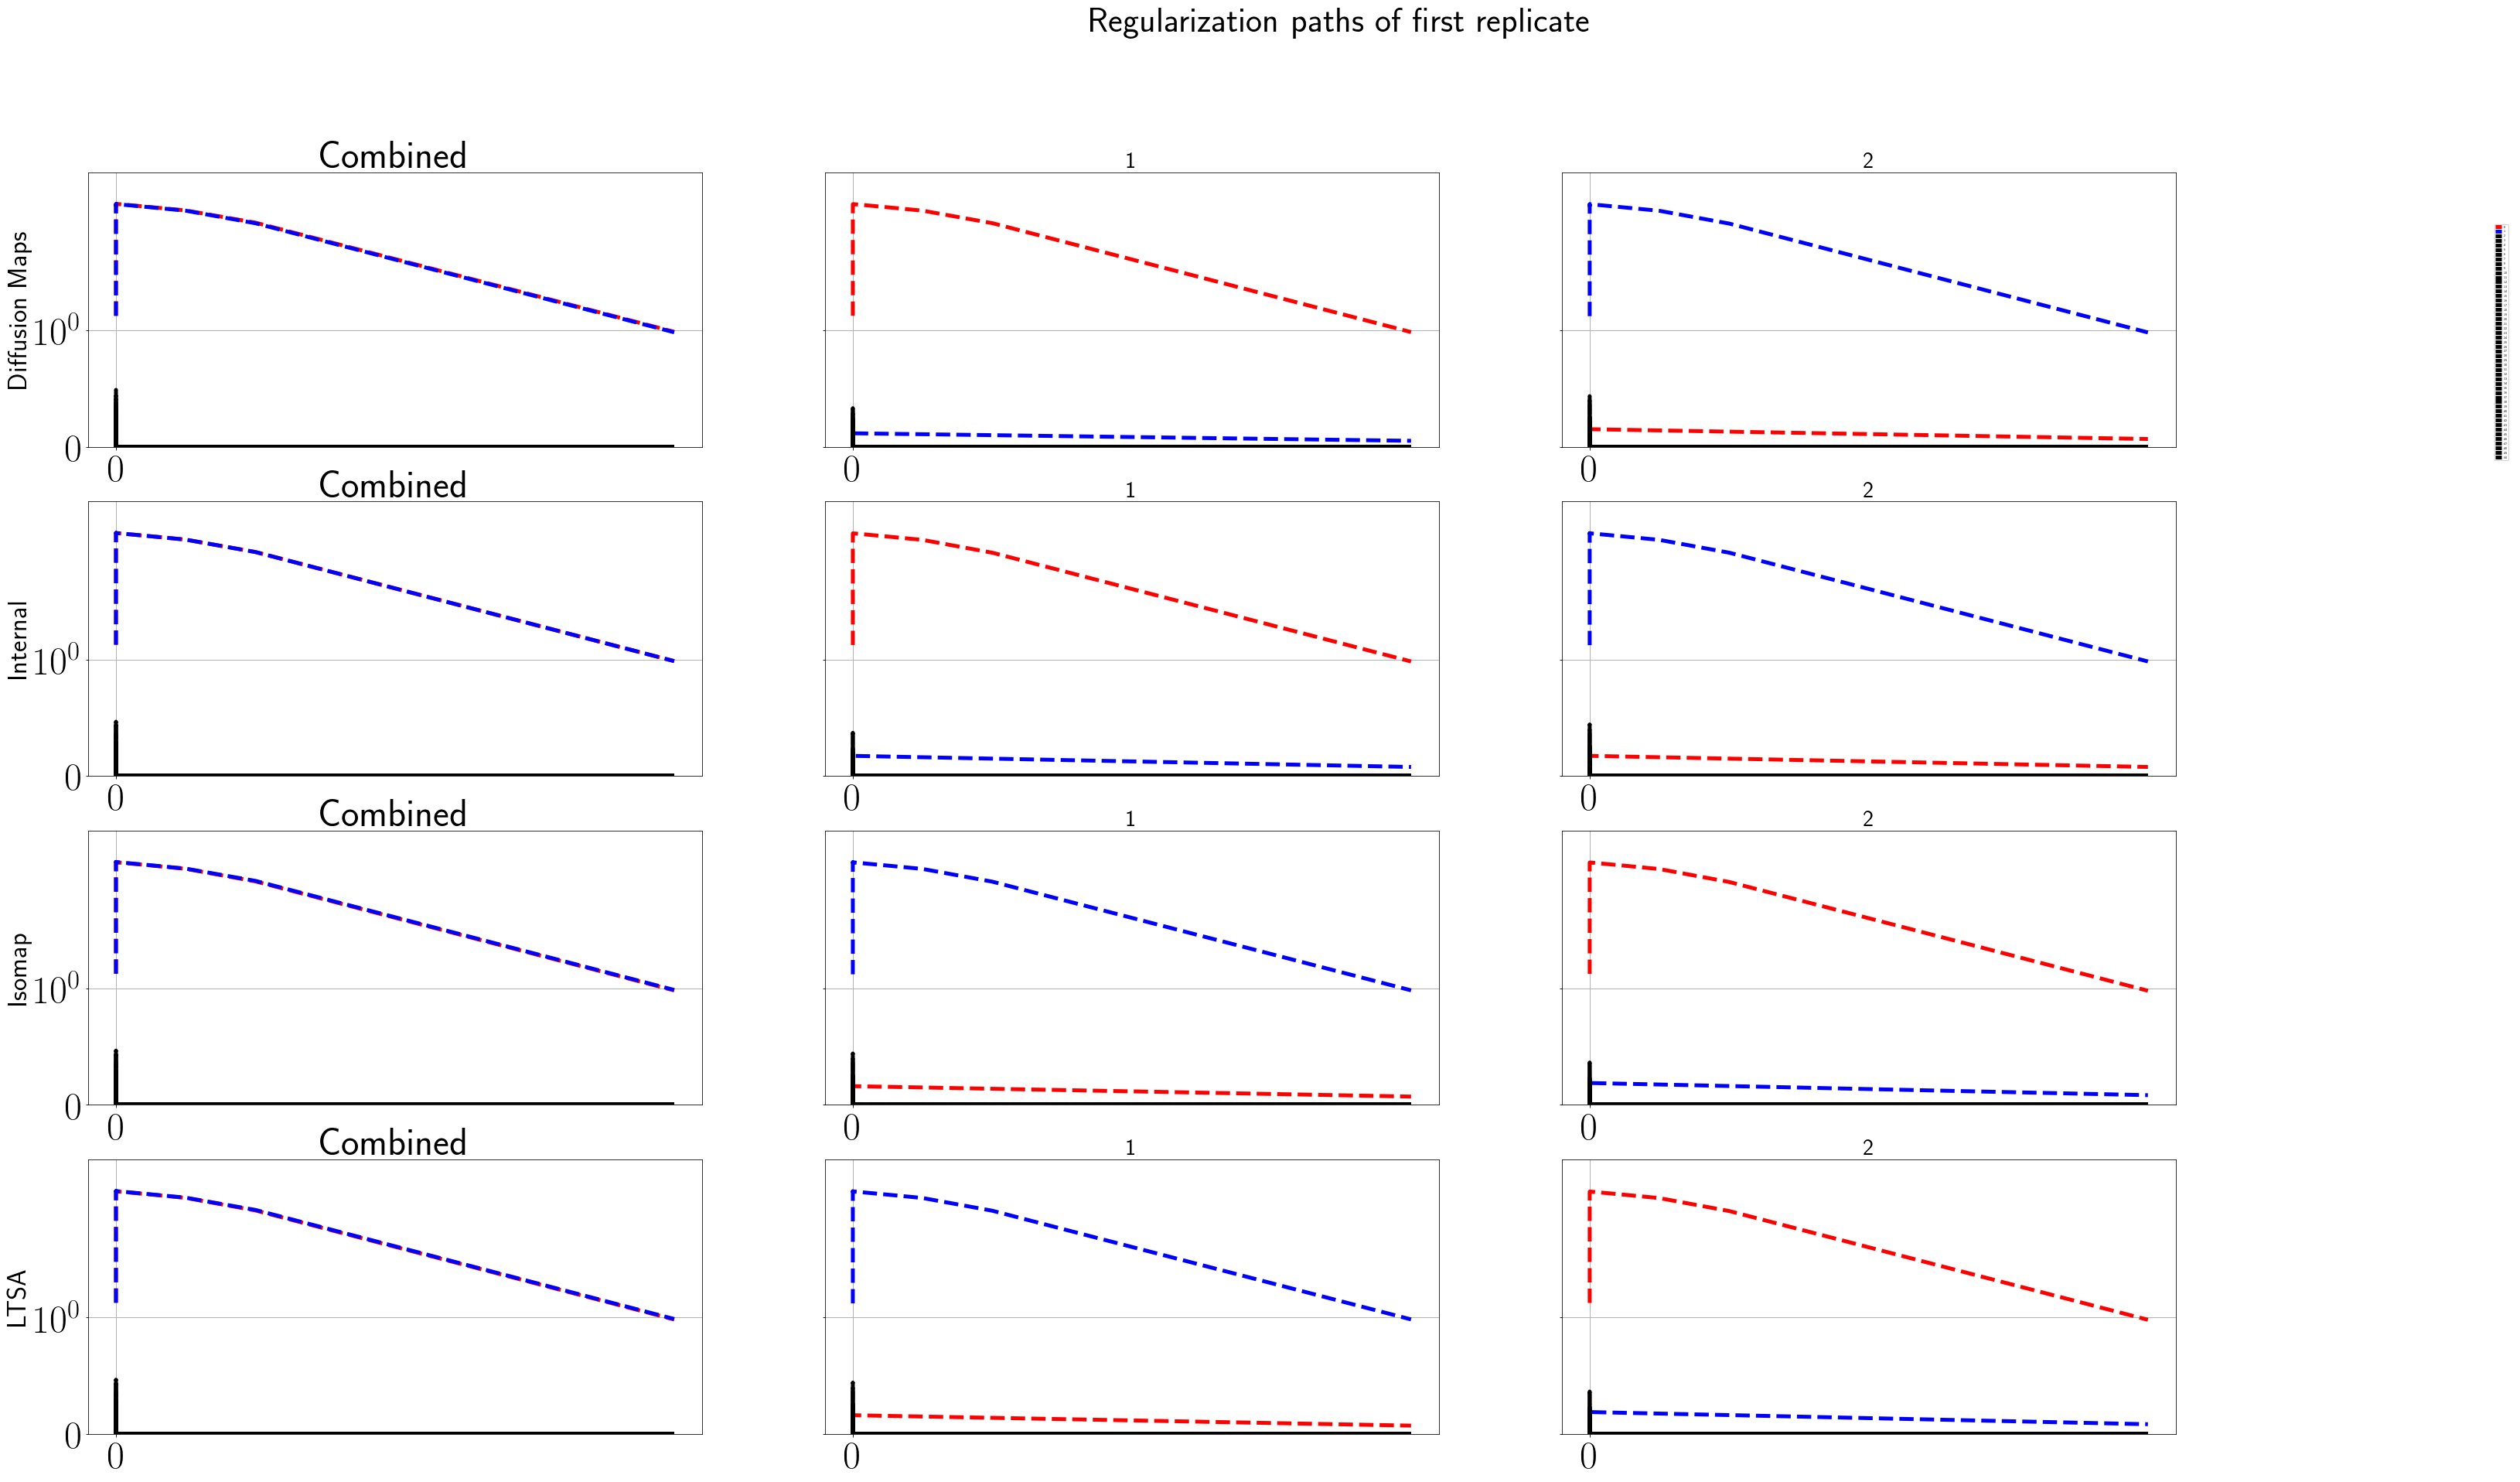
\includegraphics[width = \textwidth]{../Figures/revision_temp/swissroll}
\label{fig:sw} &
&
\end{tabular}
\caption{\skcomment{a) Embeddings of the \srdata dataset.}  b) \srdata~ \ref{fig:sw1} This figure displays the results of one replicate of \ouralg~ for several different embeddings of the \srdata dataset. The left panels displays $||\beta_{1:p}||_2$ as a function of the regularization parameter $\lambda$. The remaining panels display, each for one of the embedding coordinates $\phi_k$, the norm of the vector $\vec(\beta_{i,j,k},\,i=1:n')$ \skcomment{c) Support recovery heatmaps or equivalent.}.
%To be able to include the extreme cases $\lambda=0$ (no regularization) and $\beta_j \equiv 0$ ($j$ excluded from $S$), both figure axes are linear from 0 to 1, and logarithmic for values larger than 1. Error bars summarize the outcomes of the $\omega$ repetitions.
% \ouralg~ selects the internal coordinates over the coordinates of the ambient space for $\lambda \in [1,10]$.
 }
\end{figure}

\paragraph{\ouralg~on a Rigid Ethanol skeleton}\label{sec:rigid}

We demonstrate the efficacy of our method for molecule-type data in a controlled setting by applying it to a simple rigidly-rotating ethanol trajectory.  We first construct an ethanol skeleton composed of the atoms shown in Figure \ref{fig:ethanol-bonds}.  We then sample as we rotate the atoms around the C-C and C-O bonds, giving the simulated trajectory two a priori known degrees of freedom. These two angles are distributed uniformly over grid. This contrasts with the MD-trajectories, which are simulated according to quantum dynamics.
The dictionary (Figure \ref{figtab:eth} in Appendix \ref{app:dictionary-details}) consists of the twelve torsions implicitly defined by the bond diagram. \skcomment{should add spurious torsions. all angles?}.  Figure \ref{fig:ret3} presents the results.  

%, $g_1,g_2$ which correspond respectively to the C-C and C-O bonds marked in Figure \ref{fig:ethanol-bonds}, and two other torsions that by construction do not vary across the manifold.

\comment{Figures \ref{fig:ret1} and \ref{fig:ret2} show the estimated manifold is a two-dimensional surface with a torus topology similar to that observed for the MDS ethanol in Figure \ref{fig:molecs}. As in the MD ethanol, bond torsions $g_1$ and $g_2$ appear to parameterize the manifold. These are the two C-C and C-O torsions which vary by construction in this simulation.}

\ouralg~ identifies pairs of torsions that explain the manifold. These can be visually verified as in Figure \ref{fig:ret1} and \ref{fig:ret2}.  Figure \ref{fig:ret3} shows that, across replicates, \ouralg~ selects pairs of functions with orthogonal gradients out of the colinear functions \skcomment{Overlay selection on cosines?} . Inspecting individual replicates in Figure \ref{fig:ret4}, we can see that these associate particular dictionary elements with particular embedding coordinates that corroborates what we can visually observe in Figure \ref{fig:ret1} and \ref{fig:ret2}, and that the spurious dictionary functions are quickly eliminated.   

%
\begin{figure}[hbt!]
\begin{tabular}{ccc}
\subfloat[$g_1$]{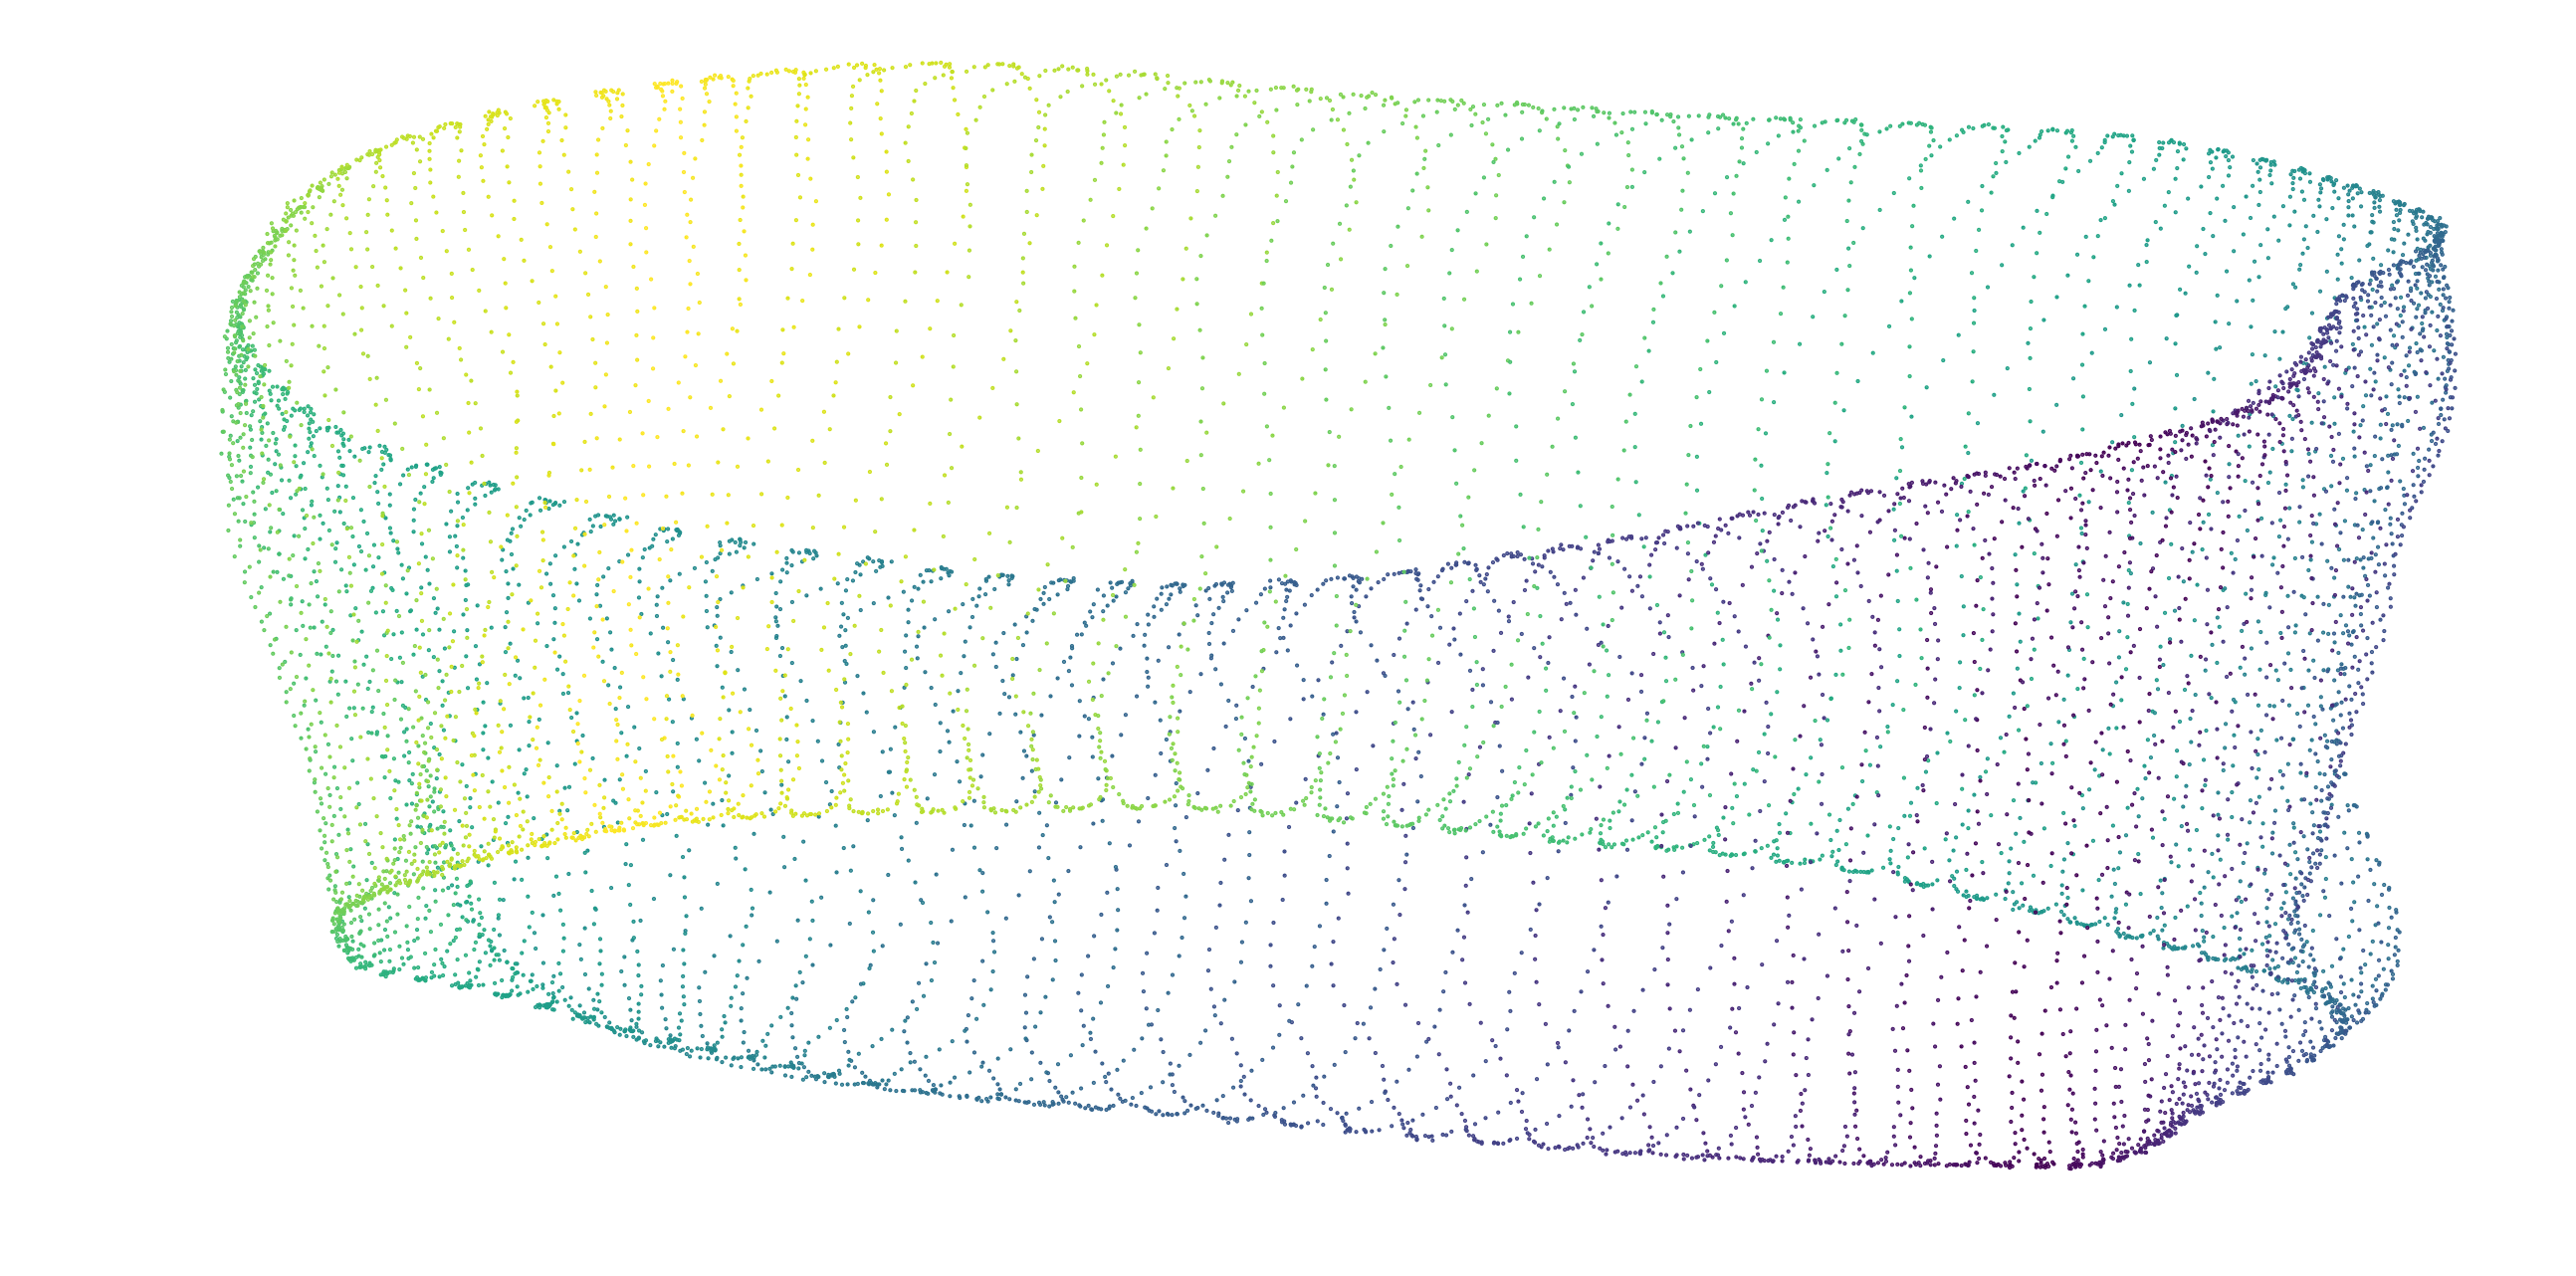
\includegraphics[width = 1in]{../Figures/rigidethanol/April_04_2019_12_51_31/torsion0.png} \label{fig:ret1}}& 
\subfloat[$g_2$]{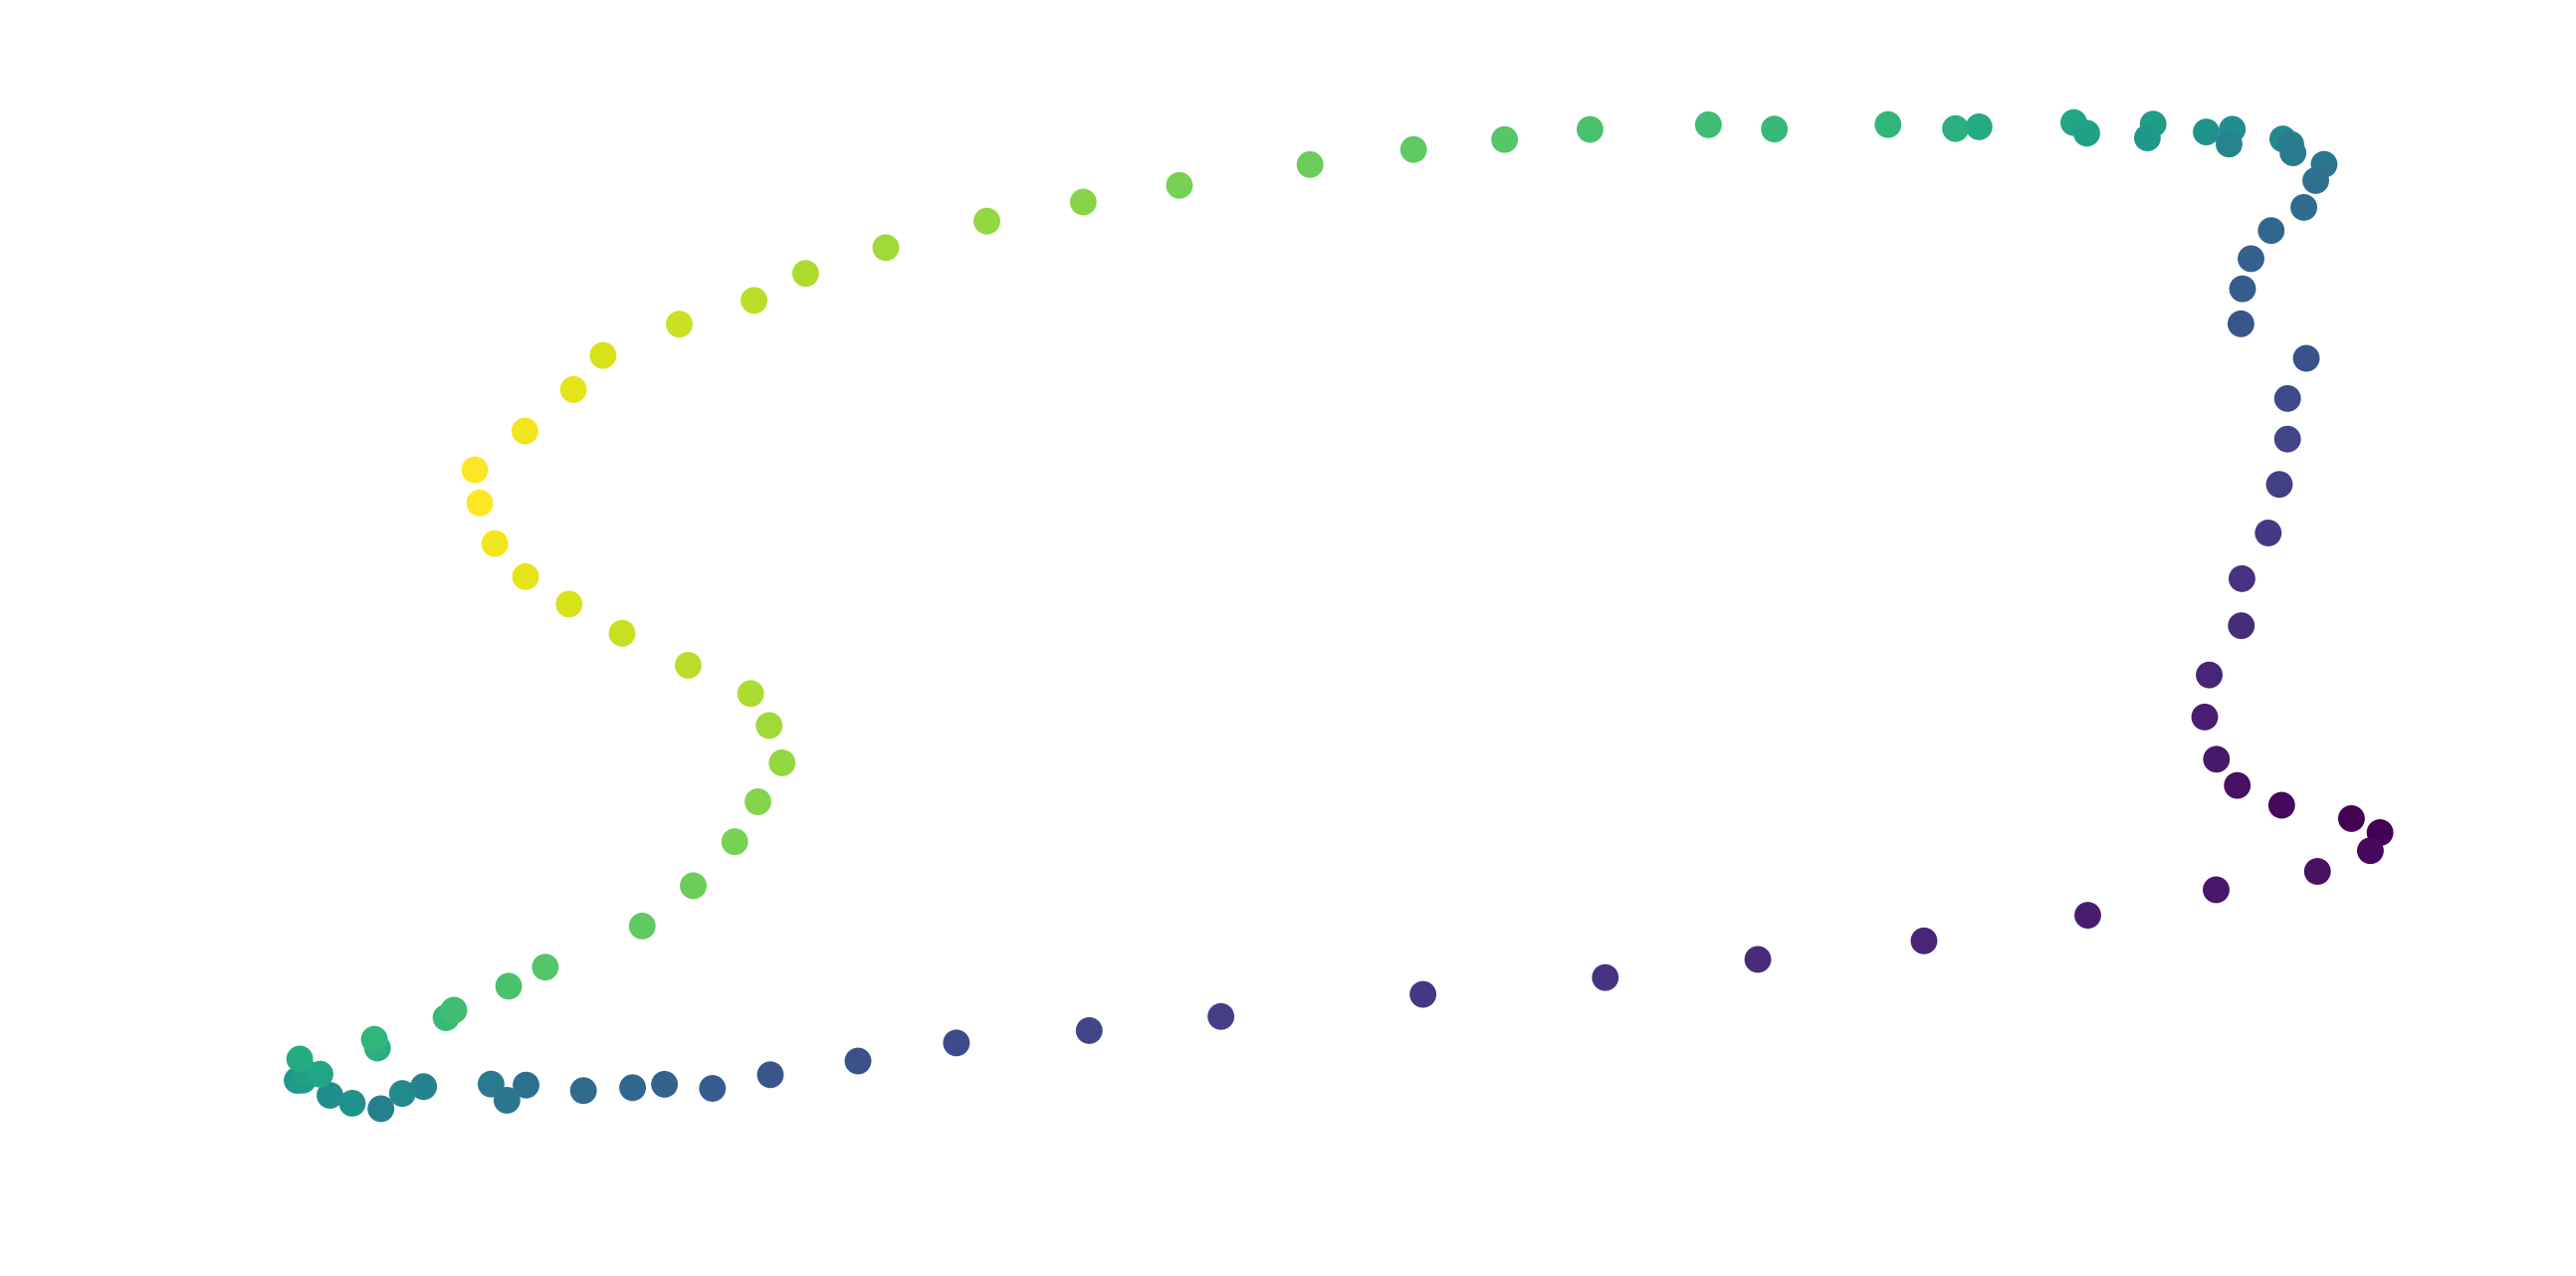
\includegraphics[width = 1in]{../Figures/rigidethanol/April_04_2019_12_51_31/torsion1.png} \label{fig:ret2}} &
 \subfloat[]{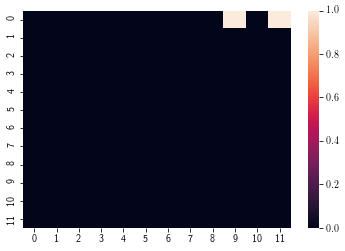
\includegraphics[width = 1in]{../Figures/revision_temp/support_recovery_temp.png} \label{fig:ret3}} \\
 \multicolumn{3}{c}{\subfloat[] {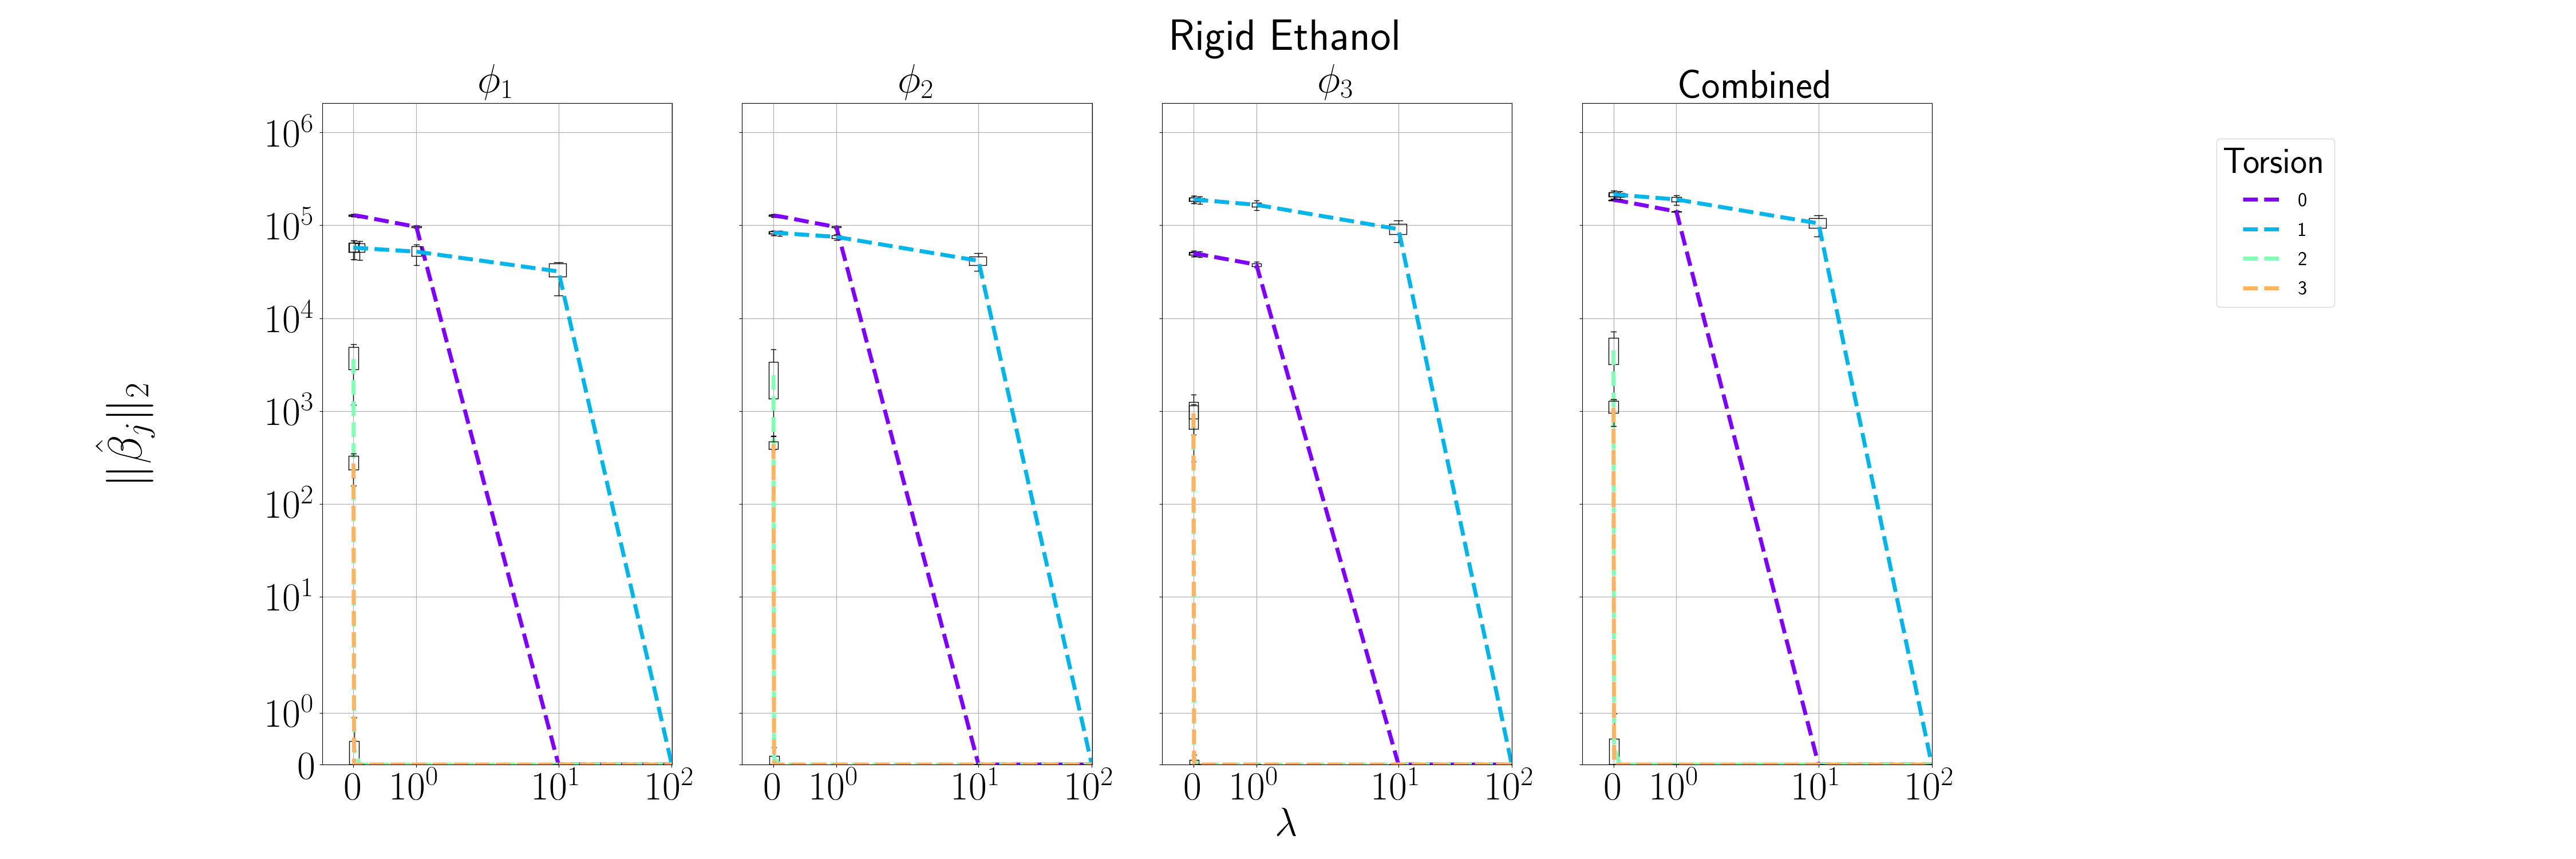
\includegraphics[width = 5in]{../Figures/rigidethanol/April_04_2019_15_15_12/betassymlogbeta_paths_log_n10000nsel100nrepss3rigidcombotoohighiter.png}} \label{fig:ret4}}
%\multicolumn{3}{*}{\subfloat[] 
\end{tabular}
\caption{\redata~ \ref{fig:ret1} The learned manifold colored by the C-C bond torsion $g_1$, the purple bond in Figure \ref{fig:ethanol-bonds}; compare this embedding with the embedding of MD ethanol in Figure \ref{fig:molecs}. \ref{fig:ret2} A radial slice of the embedding colored by the C-O bond torsion $g_2$, the blue bond in Figure \ref{fig:ethanol-bonds}. \ref{fig:ret3} This figure presents the frequency of support recovery across pairs of dictionary elements and replicates. \ref{fig:ret4} Support recovery results for one replicate of \ouralg \skcomment{This is a stand in}. 
%The left panel displays $||\beta_{1:p}||$ as a function of the regularization parameter $\lambda$. The remaining panels display, each for one of the embedding coordinates $\phi_k$, the norm of the vector $\vec(\beta_{i,j,k},\,i=1:n')$. These panels show the relative contribution of each dictionary function to explaining a particular embedding coordinate $\phi_k$. For $\lambda > 1$, $\phi_{1,2}$ are explained by $g_1$, while $\phi_3$ is explained by $g_2$. Axes are linear between $0$ and $1$, and logarithmic above $1$. Error bars summarize the outcomes of the $\omega$ repetitions.
}
\label{fig:rigid-ethanol}
\end{figure}

\subsection{Molecular Dynamics Data}\label{sec:mds_data}

\paragraph{Ethanol}\label{sec:ethanol}

%Ethanol has no p-orbital hybridization, and a more intricate vibrational structure than toluene.
Figure \ref{fig:molecs} shows that the estimated manifold is a two-dimensional toroidal surface, and that the two generators of the torus corresponds to bond torsions $g_1$ and $g_2$.  Our dictionary consists of these two torsions, as well as two other dihedral angles. \ouralg~ identifies that $g_1$ and $g_2$ explain the manifold. Furthermore, it associates $g_1$ with embedding coordinates $\phi_1$ and $\phi_2$ and $g_2$ with $\phi_3$, which reflects the orientation of the generators in the Figure.

%
\begin{figure}[H]
\setlength{\picwi}{0.3\llw}
\begin{tabular}{ccc}
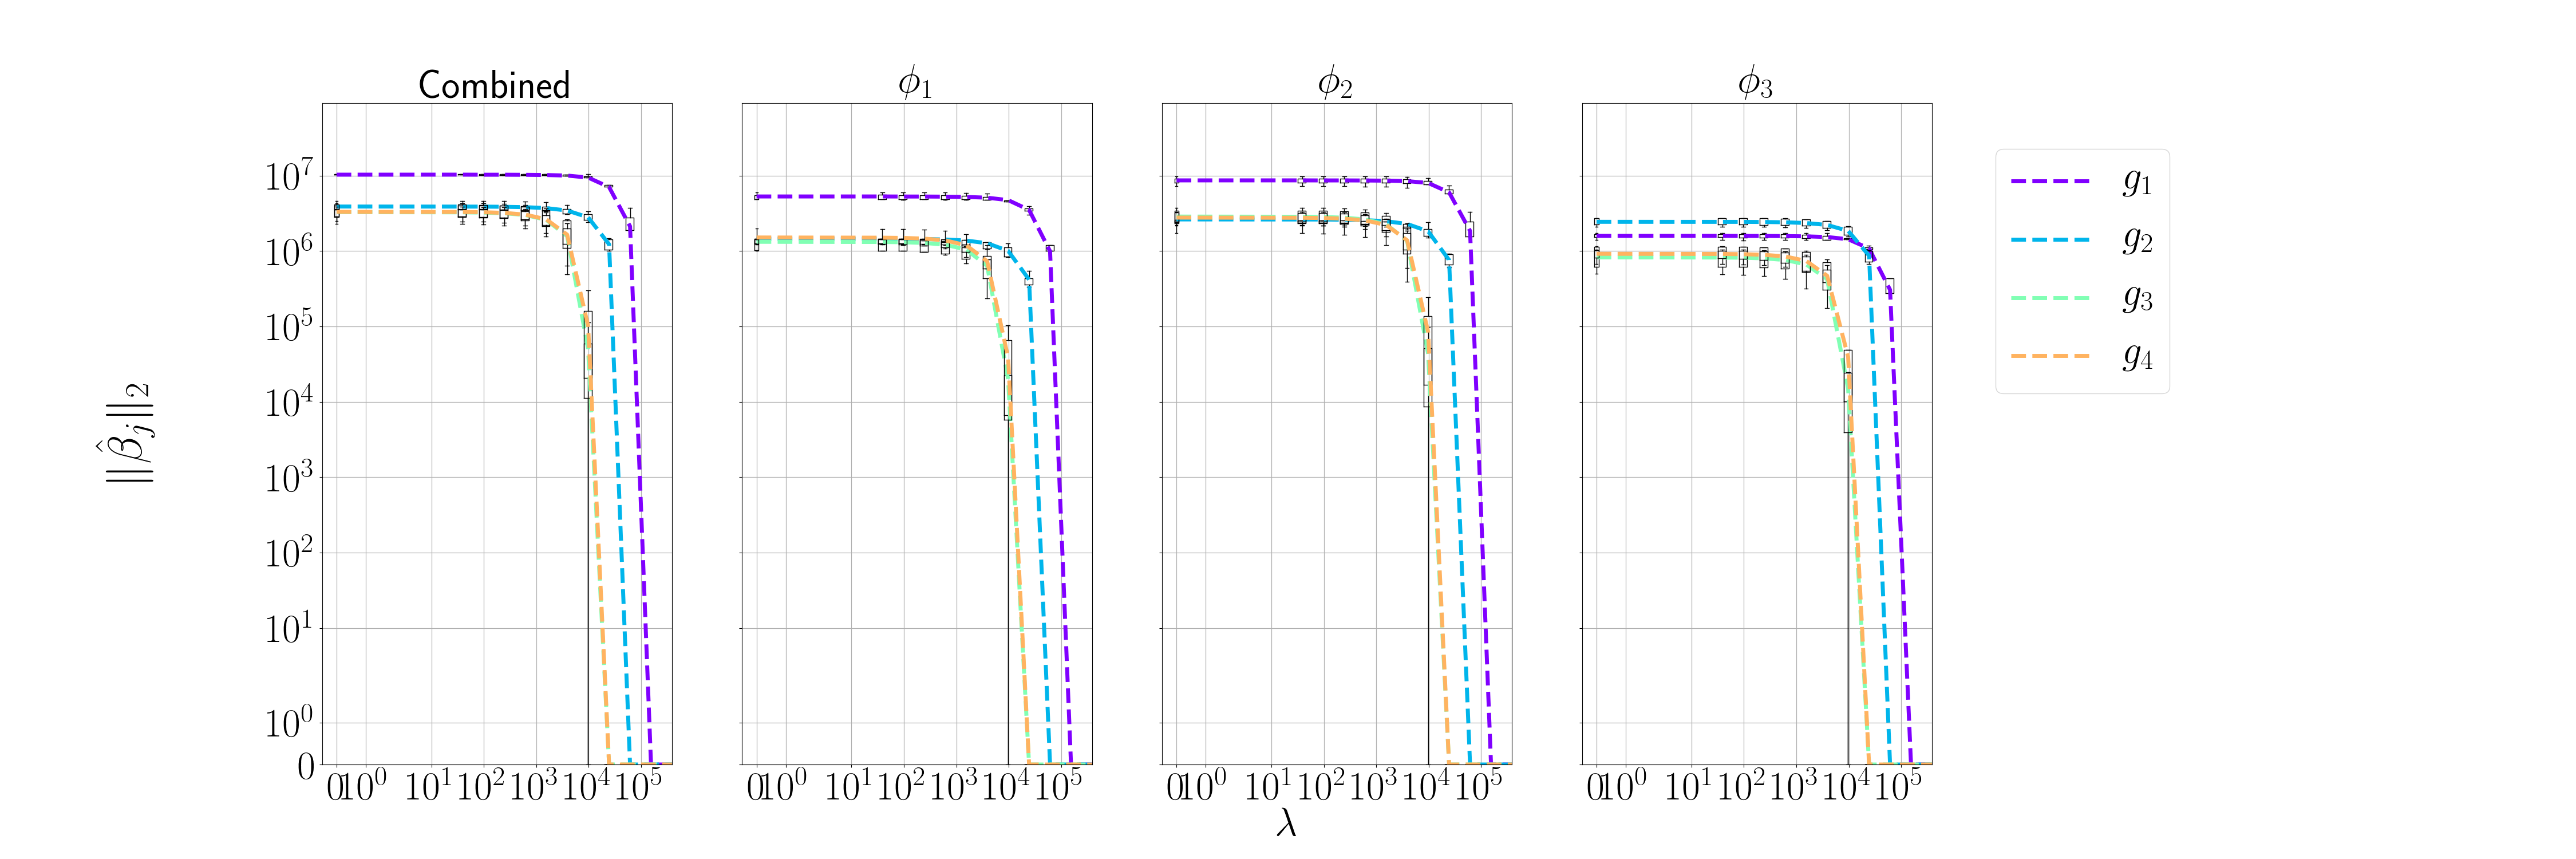
\includegraphics[width=4\picwi,height=1.5\picwi]{../Figures/ethanol/June_27_2019_17_17_08/betassymlogsymlogbeta_paths_n50000nsel100nreps5.png}
\end{tabular}
\caption{\ethdata~ The left panel displays $||\beta_{1:p}||$ as a function of the regularization parameter $\lambda$. The remaining panels display, each for one of the embedding coordinates $\phi_k$, the norm of the vector $\vec(\beta_{i,j,k},\,i=1:n')$. For $\lambda > 10^4$, $\phi_{1,2}$ are explained by $g_1$, while $\phi_3$ is explained by $g_2$. Note that some preference is given to $g_2$ by $\phi_3$, and that this corresponds to the embedding that we see in Figure \ref{fig:molecs}. Axes are linear between $0$ and $1$, and logarithmic above $1$. Error bars summarize the outcomes of the $\omega$ repetitions.
}
\label{fig:mds-ethanol}  
\end{figure}

\paragraph{Malonaldehyde}\label{sec:malonaldehyde}

\begin{figure}[H]
\setlength{\picwi}{0.3\llw}
\begin{tabular}{ccc}
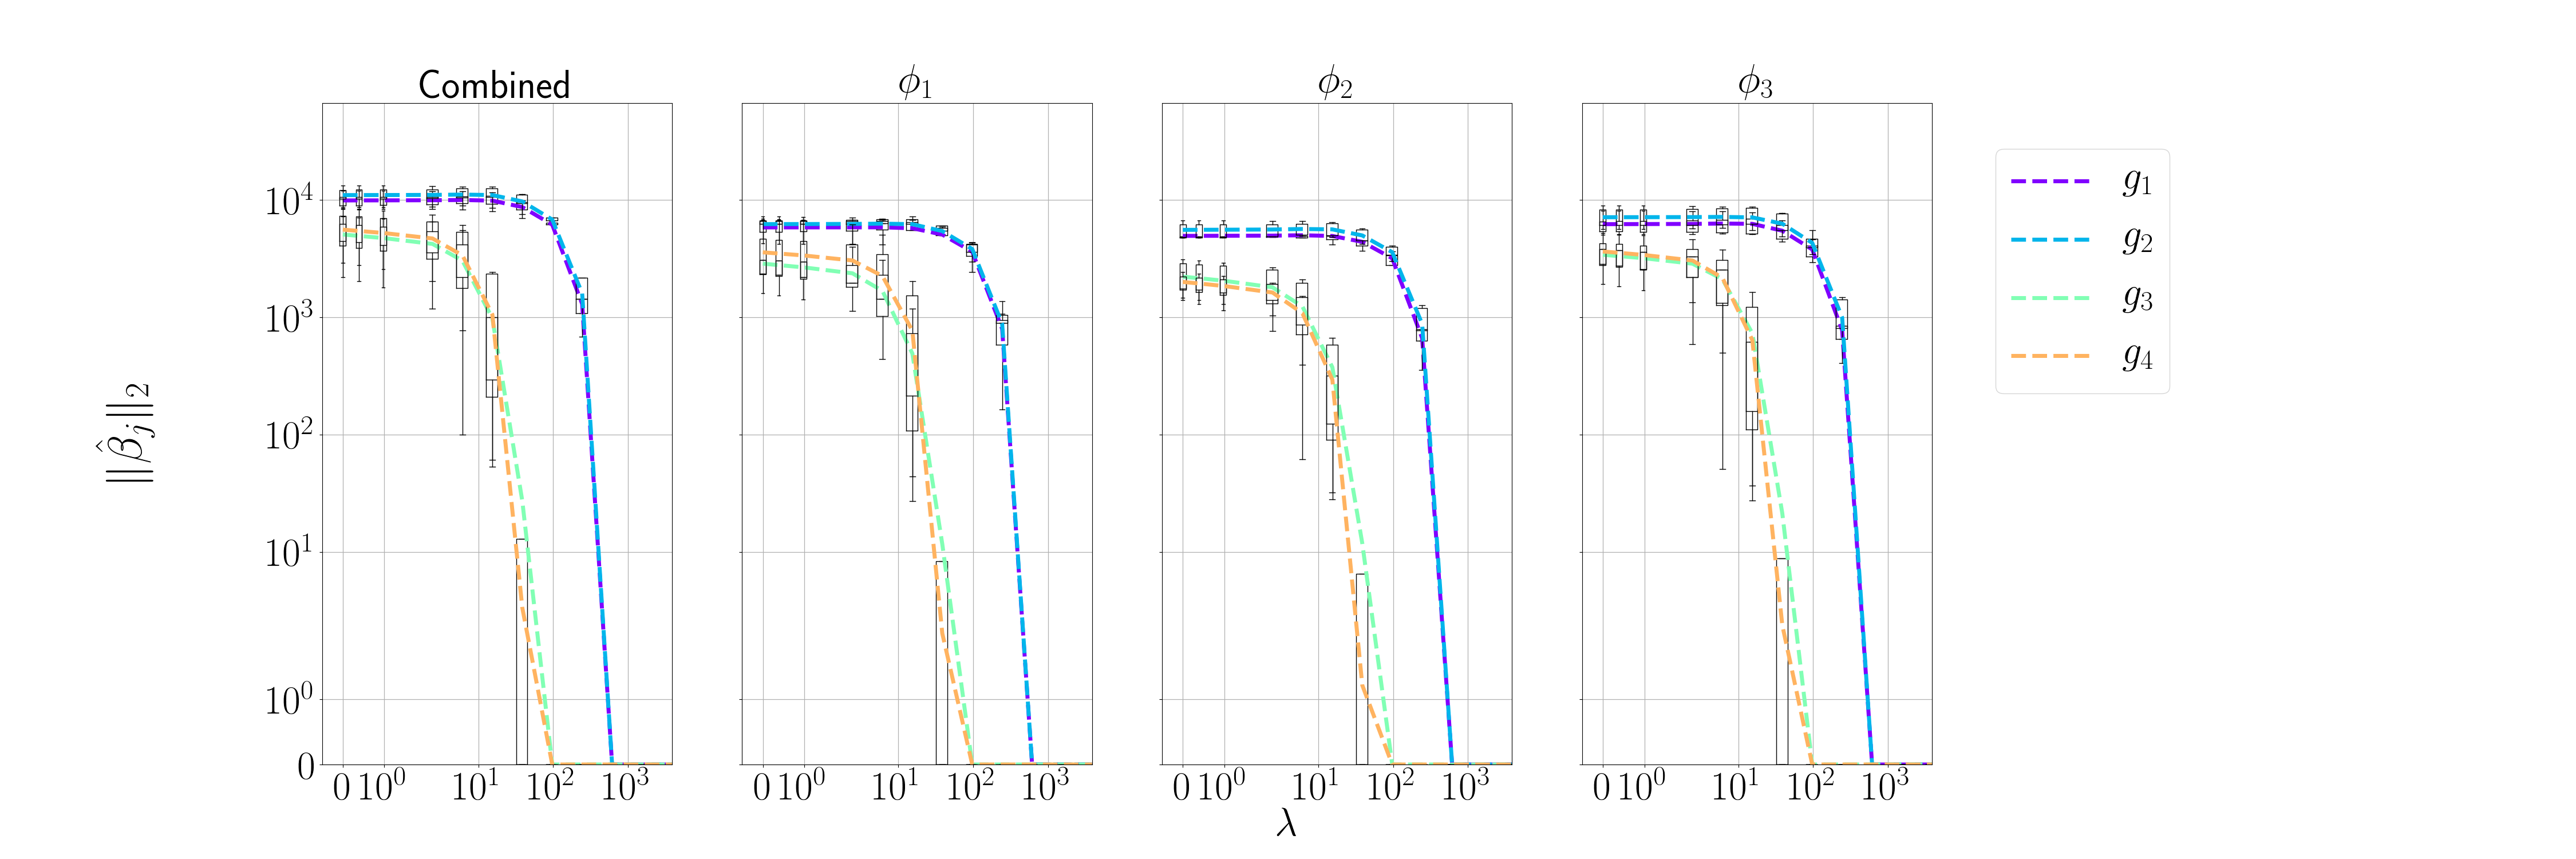
\includegraphics[width=4\picwi,height=1.5\picwi]{../Figures/malonaldehyde/June_27_2019_17_24_21/betassymlogsymlogbeta_paths_n50000nsel50nreps5.png}
\end{tabular}
\caption{\maldata~ The left panel displays $||\beta_{1:p}||$ as a function of the regularization parameter $\lambda$. The remaining panels display, each for one of the embedding coordinates $\phi_k$, the norm of the vector $\vec(\beta_{i,j,k},\,i=1:n')$. For $\lambda > 10^2$, $\phi_{1,2,3}$ are explained by $g_{1:2}$. This corresponds to the embedding that we see in Figure \ref{fig:molecs}. Axes are linear between $0$ and $1$, and logarithmic above $1$. Error bars summarize the outcomes of the $\omega$ repetitions.
\label{fig:mds-malonaldehydel} }
\end{figure}

%Malonaldehyde has a slightly more complex structure than ethanol, with possible p-orbital hybridization between the two oxygen atoms.

Figure \ref{fig:molecs} shows that the estimated manifold is a two-dimensional surface on which bond torsions $g_1$ and $g_2$ vary smoothly. Our dictionary consists of these two torsions, as well as two other dihedral angles. \ouralg~ identifies that $g_1$ and $g_2$ explain the manifold. In contrast to ethanol and rigid ethanol, all coordinates are associated indistinguishably with both functions.

%\mmp{to merge if needed}

\paragraph{Toluene}\label{sec:toluene}
%Toluene is a simple small molecule with one rotational degree of freedom.  P-orbital hybridization keeps the benzene ring and its peripheral hydrogens locked in a planar configuration, while the CH3 methyl group can rotate freely.

Figure \ref{fig:molecs} shows that the estimated manifold is a circle parameterized by the $CH_3$ methyl torsion $g_1$.  Our dictionary consists of this angle, as well as other dihedral angles throughout the molecule. \ouralg~  identifies that $g_1$ explains the manifold, and associates both coordinates with this function. 
 It is easy
to see that the the \dpullalg~maps tangent vectors from the embedding
space back to the correct subspace.

%In contrast to the setting in the previous section, we have no a priori knowledge of the shape of the data manifold. We can visually check that this circle corresponds to a bond torsion of the methyl group.

%\ouralg~ provide a statistically validated alternative to this visual inspection method.
\begin{figure}[H]
\setlength{\picwi}{0.3\llw}
\begin{tabular}{ccc}
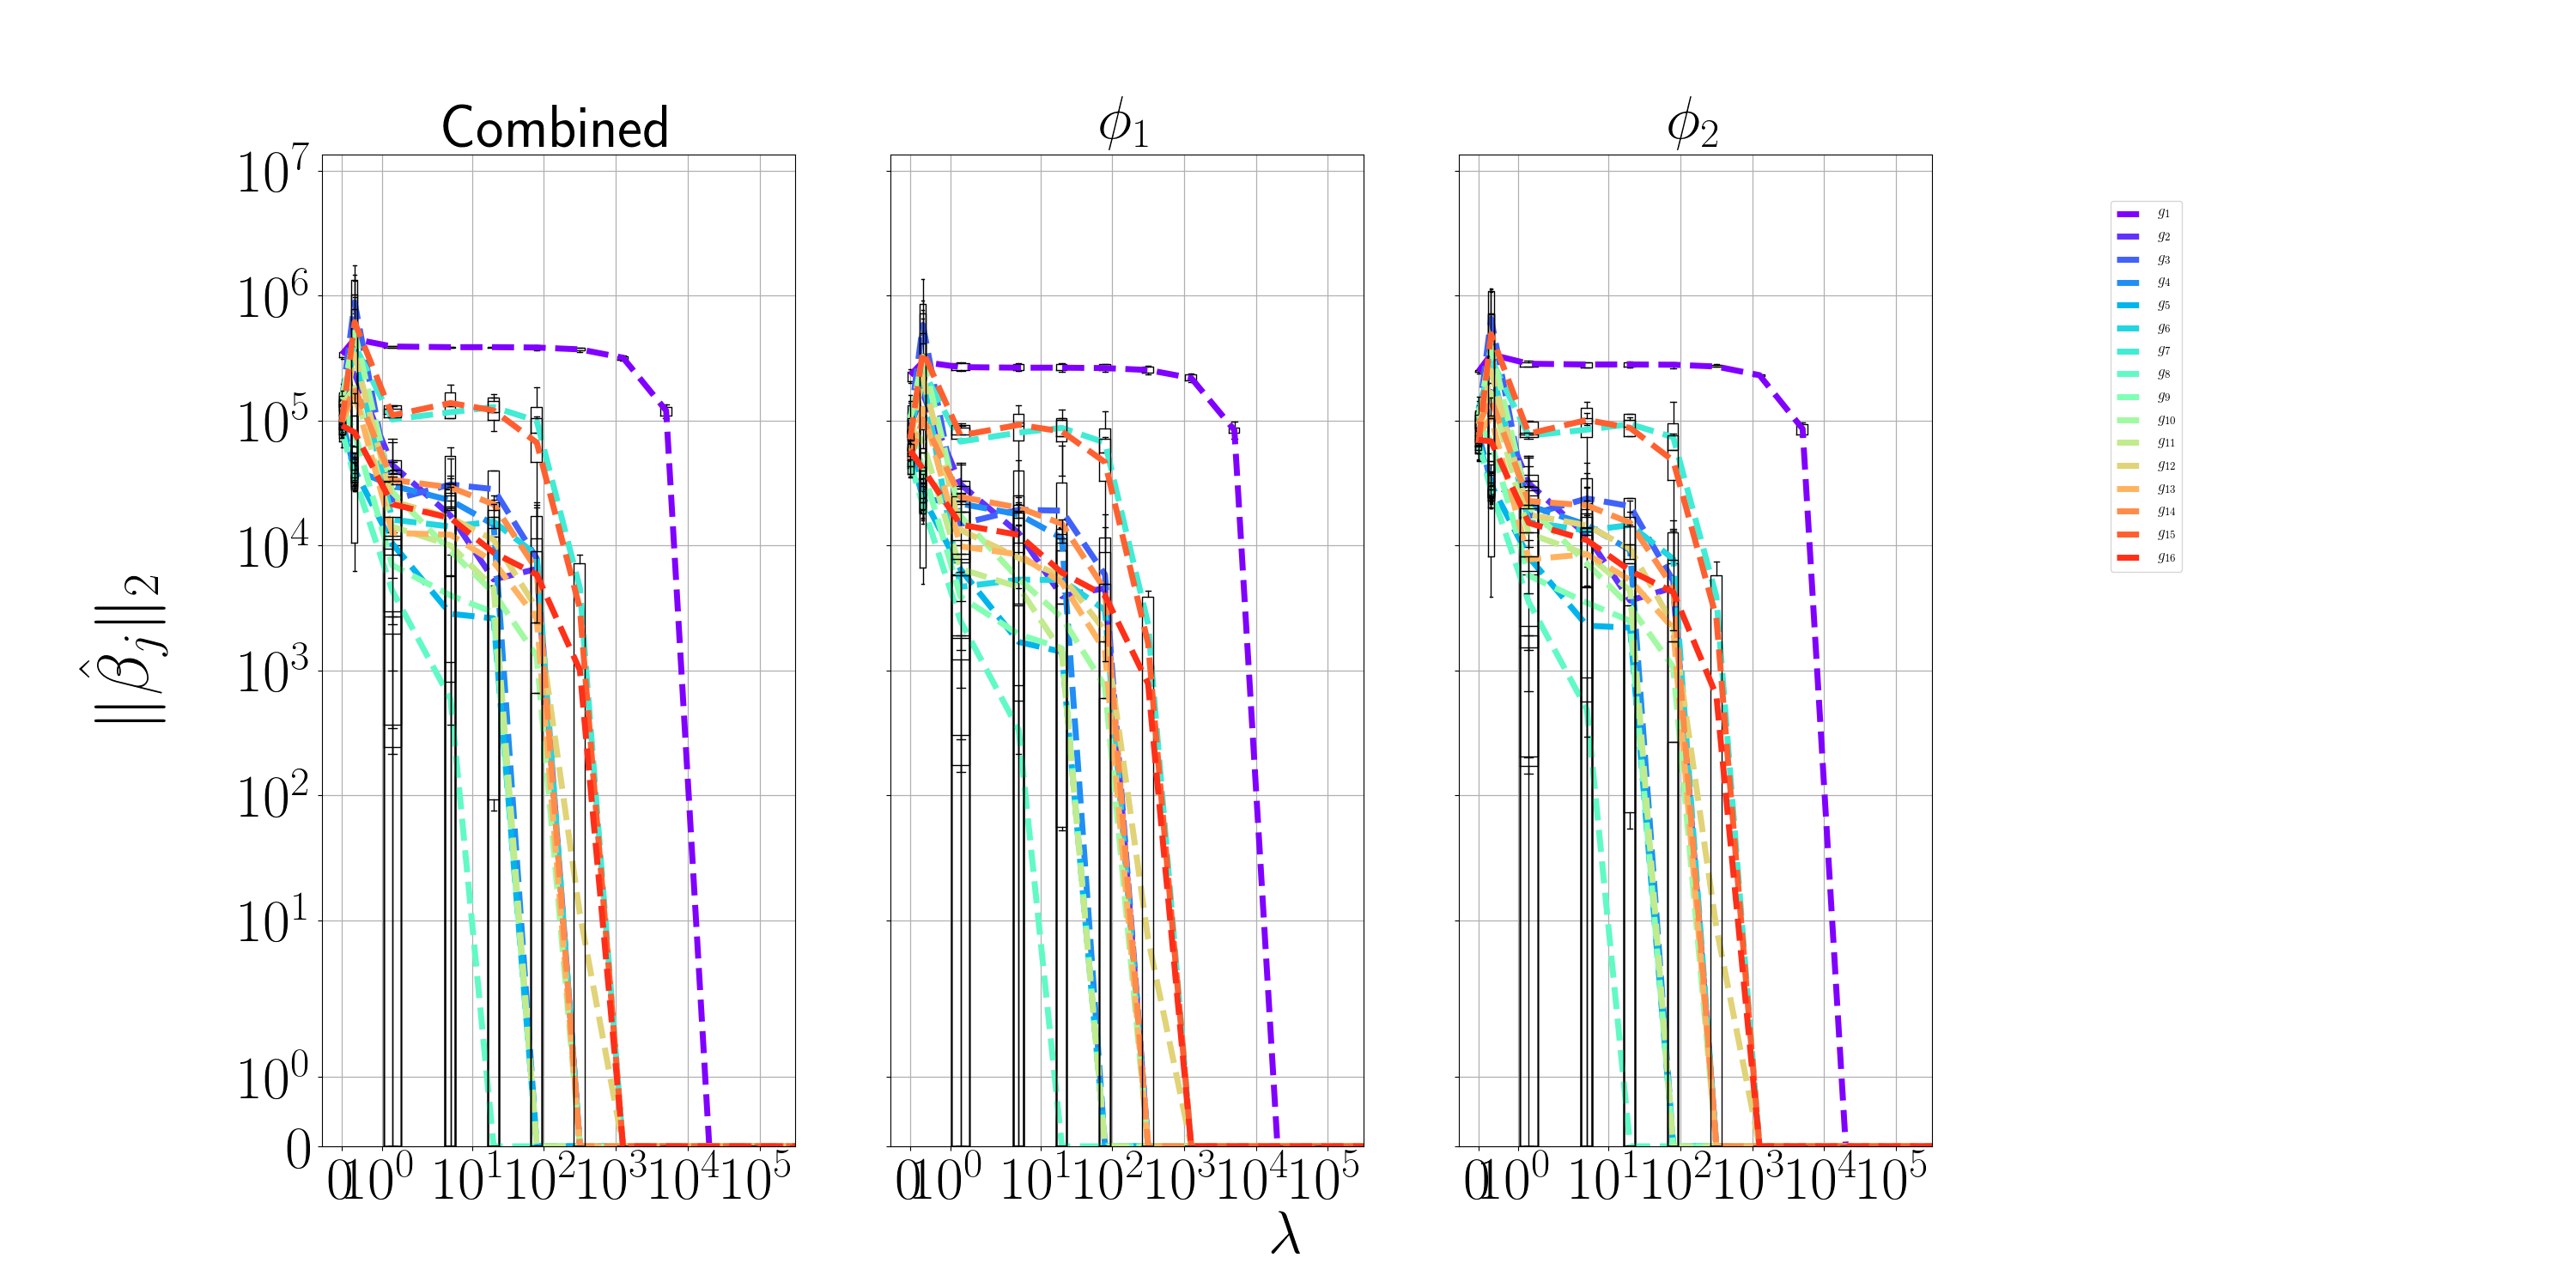
\includegraphics[width=4\picwi,height=1.5\picwi]{../Figures/toluene/June_27_2019_17_17_08/betassymlogsymlogbeta_paths_n50000nsel50nreps5.png}
\end{tabular}
\caption{\toldata~ The left panel displays $||\beta_{1:p}||$ as a function of the regularization parameter $\lambda$. The remaining panels display, each for one of the embedding coordinates $\phi_k$, the norm of the vector $\vec(\beta_{i,j,k},\,i=1:n')$. For $\lambda > 10^3$, $\phi_{1,2}$ are explained by $g_{1}$. This corresponds to the embedding that we see in Figure \ref{fig:molecs}. Axes are linear between $0$ and $1$, and logarithmic above $1$. Error bars summarize the outcomes of the $\omega$ repetitions.
}
\label{fig:mds-toluene}
\end{figure}